\chapter{Models for  Search-Encounter Data}
\markboth{Search-Encounter}{}
\label{chapt.search-encounter}

\vspace{0.3cm}


In this chapter we discuss models for search-encounter data. These
models are useful in situations where the locations of individuals,
say ${\bf u}_{ik}$ for individuals $i$ and sample occasions $k$, are
observed directly by searching space (often delineated by a polygon)
in some fashion, rather than restricted to fixed trap locations.  In
all the cases addressed in this chapter, both detection probability
and parameters related to movement can be estimated using such models.
Conversely, when we have an array of fixed trap locations, the
movement process is completely confounded with the encounter process
because the list of potential observation locations is prescribed, a
priori, indendent of any underlying movement process.  The models we
differentiate here depend on a number of things related to data
structure or survey protocol -- basically whether or not we record the
exact location and how we record it.

A few distinct types of situations exist where these models come in
handy. The prototypical, maybe ideal, situation
\citet{royle_etal:2011mee} is where we have a single search path
through a region of space from which observations are made (just as in
the typical distance sampling situation, using a transect). As we walk
along the search path, we note the location of each individual that is
detected, {\it and their identity} (this is different from distance
sampling in that sense).  Alternatively, we could delineate a search
area, and conduct a systematic search of that region. An example is
that of \citet{royle_young:2008}, which involved a plot search for
lizards. They assumed the plot was uniformly searched which justified
an assumption of constant encounter probability, $p$, for all
individuals within the plot boundaries.  The data set was $\ge 1$
location observations for each of a sample of $n$ individuals.  The
recent paper by \citet{efford:2011} discussed likelihood analysis of
similar models. In the terminology of \mbox{\tt secr} such models are
referred to as models for {\it polygon detectors}.
%The model described by \citep{royle_etal:2011mee} is a
%generalization of the polygon search model, as we describe below.
% XX RS: You also gonna describe the transect model? Might be nice to add, if so. Something like in the other chapters, like, 'in this chapter... blabla'

% XXXX RC: You might formalize some of this by saying that in standard
% SCR, we use [y|s][s] but in search-encounter we use [y|u][u|s][s]

\begin{comment}
%%## This argument here is basically true, but i'm not sure how to
%%package the idea yet.
Search-encounter models also provide something of a bridge between the
standard models for fixed trap arrays (e.g., Chapt. \ref{chapt.scr0}, etc.),
and the models described in Chapt. \ref{chapt.scr-unmarked} in which individual
identity is not available. One one hand, in the standard fixed trap
array situation, we observe individual encounter data at each fixed
trap. In the ``no ID'' models, we observe trap-specific encounter
frequencies, but no individual identity.
Search-encounter models are intermediate
in terms of the structure of the observable data.
\end{comment}


\section{Search-encounter sampling designs}

Before we discuss models for search-encounter data, we'll introduce some
types of sampling situations that produce individual location data
by searcing space.  We imagine there are a lot more sampling protocols
(and variations) than identified here, but these are some of the
standard situations that we have encountered over the last few years
in developing applications of SCR models.  For our purposes here we
recognize 4 basic sampling designs, each of which might have
variations due to modification of the basic sampling protocol.


\subsection{Design 1: Search-Encounter}
\label{searchencounter.sec.fixedpath}

A useful class of models arises when we have a continuous search-path
or line, or multiple such lines, in some region
(Fig. \ref{searchencounter.fig.snakeline}) from which individual
detections are made We assume the survey path is laid out {\it a
  priori} in some manner that is done independent of the activity
centers of individuals and the collection of data does not affect the
lines.  The purpose of this assumption, in the models described
subsequently, is to allow us to assume that the activity centers are
uniformly distributed on the prescribed state-space. Alternatively,
explicit models could be entertained to mitigate a density gradient or
covariate effects (see Chapt. \ref{chapt.state-space}). The situation
depicted in Fig. \ref{searchencounter.fig.snakeline} shows the search
path traversing several delineated polygons, although the polygon
boundaries may or may not affect the potential locations of
individuals (see below).

A number of variations of this search-encounter situation are
possible, and these produce slightly different data structures and
corresponding modifications to the model, although we do not address
all of these from a technical standpoint here:
\begin{itemize}
 \item[] Protocol (1a). We know the search path and record the
   locations of individuals. 
 \item[] Protocol (1b). We record the location of individuals and
   the location on the search path where we first observed the individual.
 \item[] Protocol (1c). We record
the closest perpendicular distance. This is a typical
   distance sampling situation, and this is a type of hybrid
   SCR/distance sampling model. 
 \end{itemize}

\begin{figure}
\centering
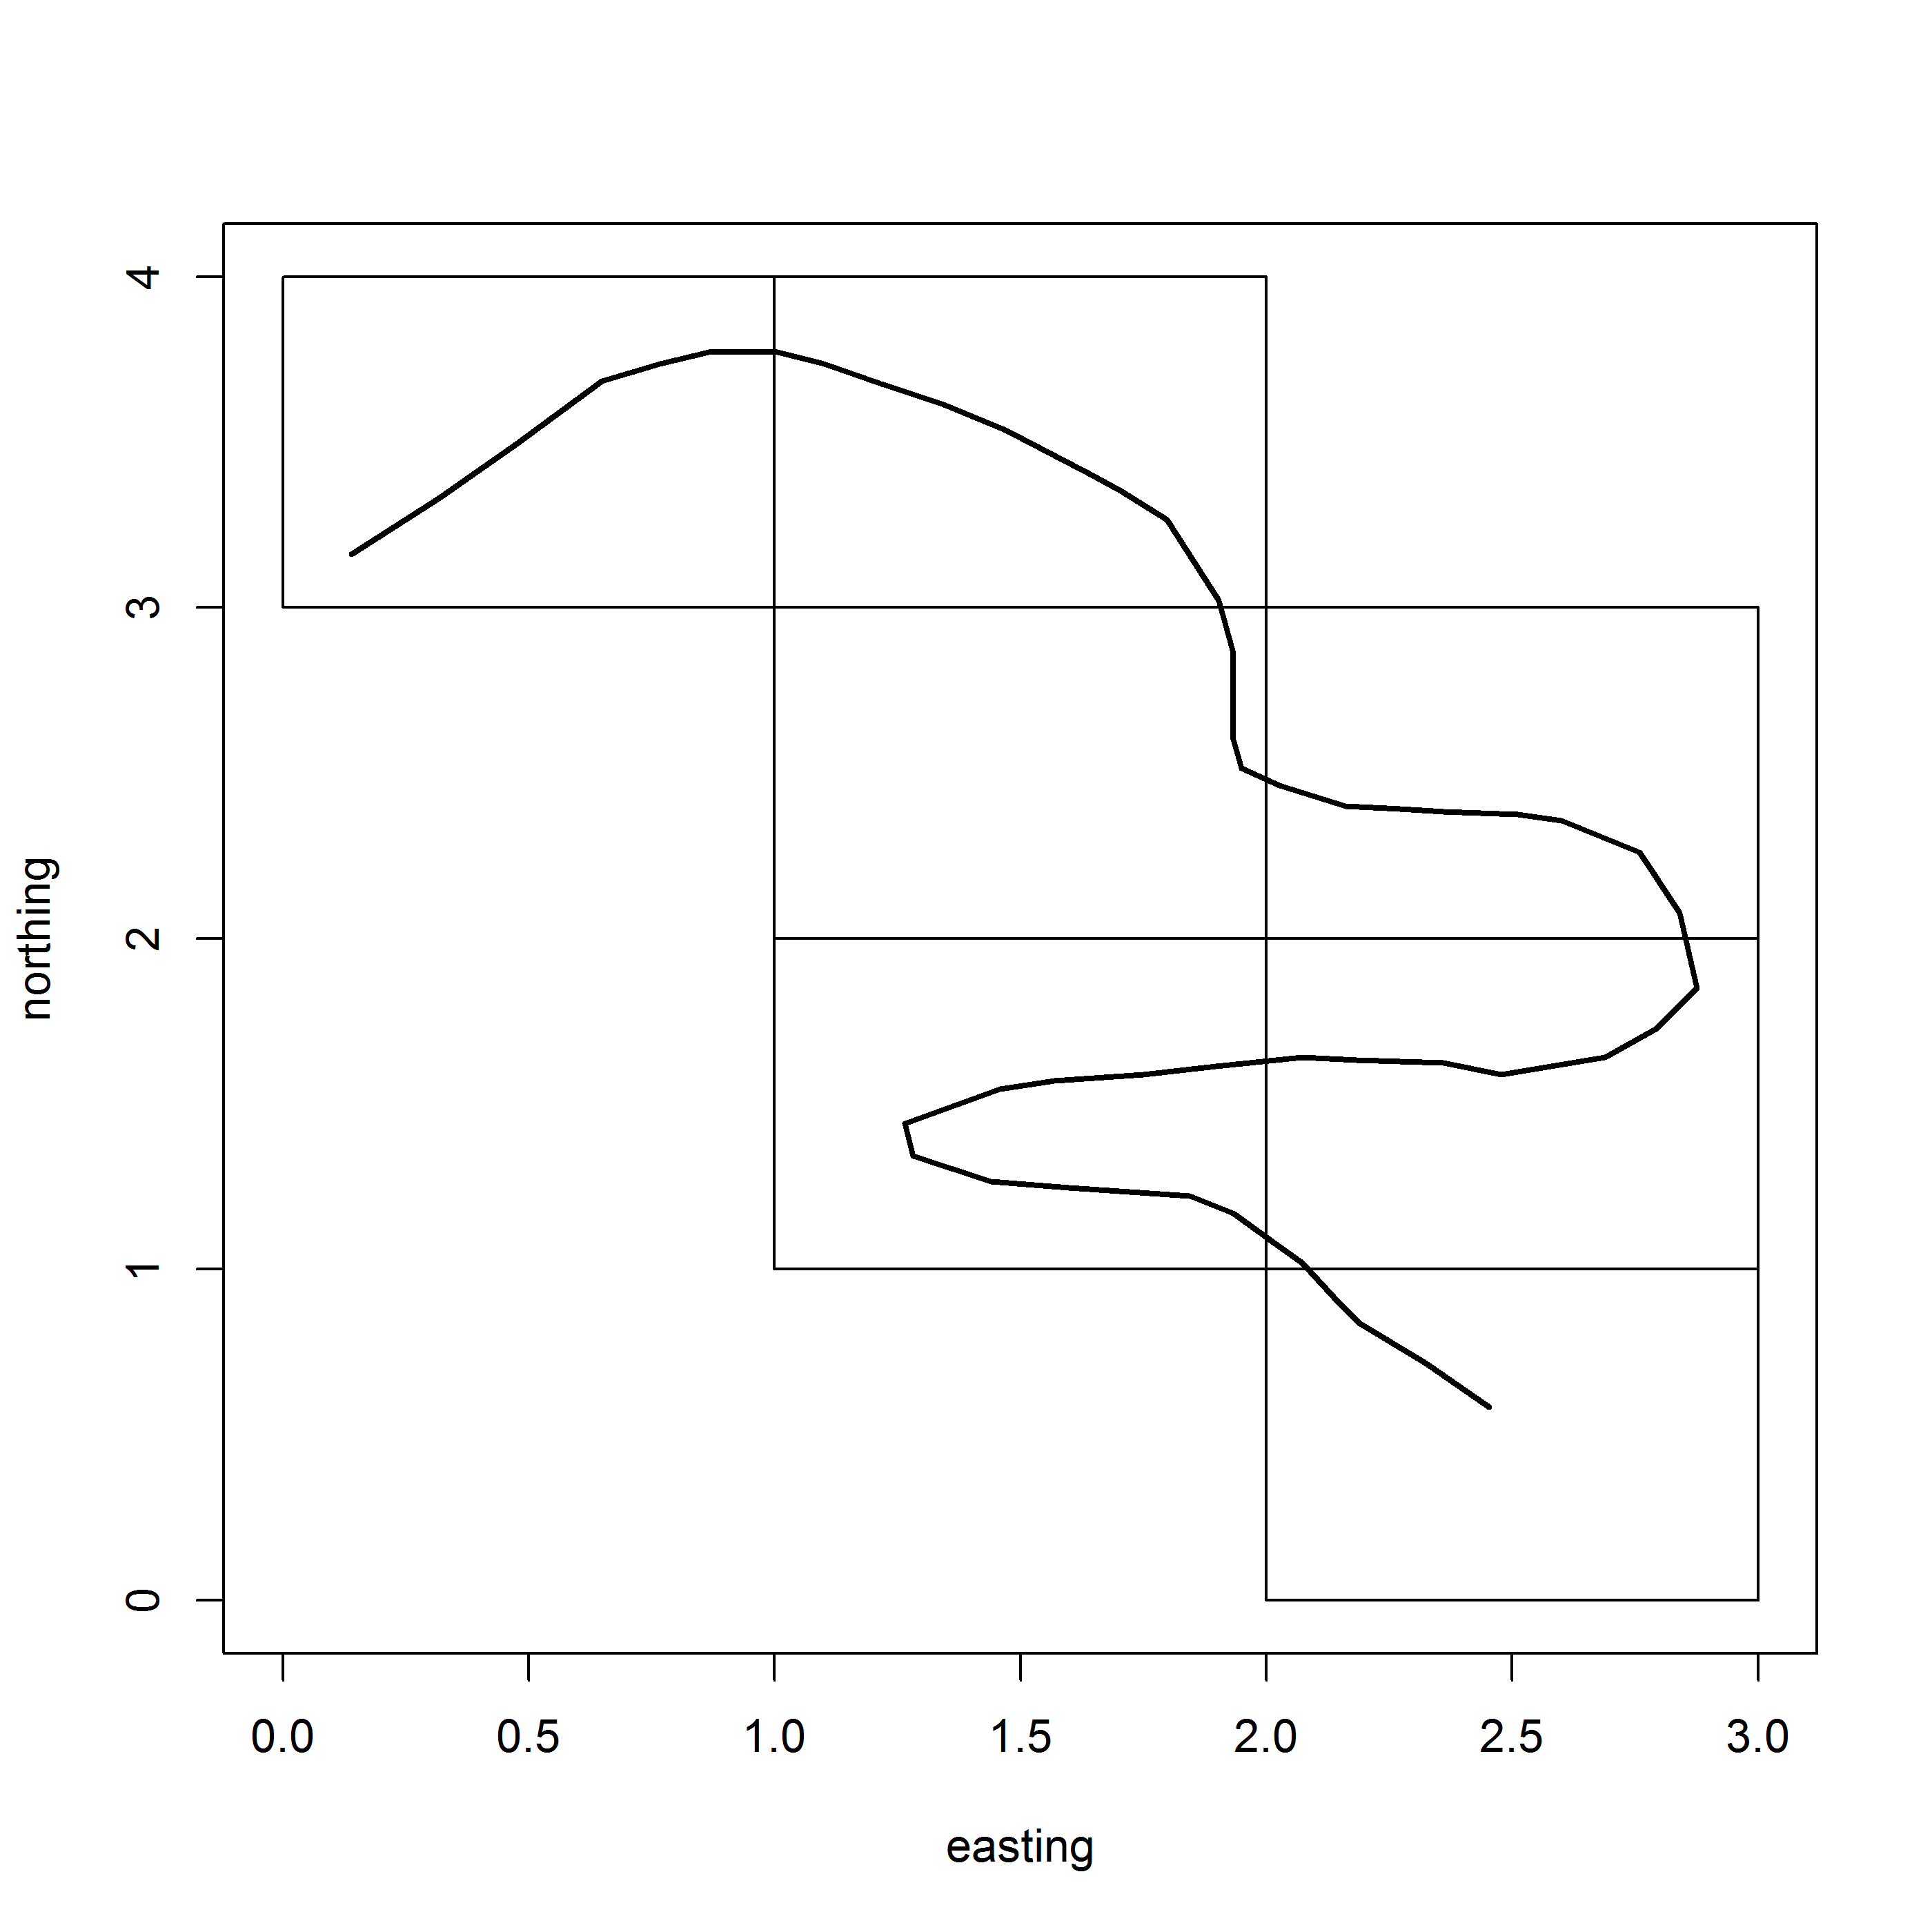
\includegraphics[width=3.5in,height=3.5in]{Ch15-searchencounter/figs/snakeline.png}
\caption{
A survey line through parts of 7 quadrats in a
  hypothetical landscape. An observer travels the transect and
  identifies individuals in the vicinity of the line, recording their
  identity and location.
}
\label{searchencounter.fig.snakeline}
\end{figure}


\subsection{Design 2: Uniform search intensity}

In the uniform search intensity model (or just ``uniform search''), we
have one or more well-defined sample areas (polygons), such as a
quadrat or a transect, and we imagine that the area is uniformly
searched so that encounter probability is constant for all individuals
within the search area.  This type of sampling method is often called
``area search'' in the bird literature \citep{bibby_etal:1992}.
Sampling produces locations of individuals within the well-defined
boundaries of the sample area. The polygon boundaries defining the
sample unit are important because they tell us that $p=0$ by design
outside of the boundary.

Using the example from the Fig. \ref{searchencounter.fig.snakeline},
but ignoring the survey line through the plot (pretend it doesn't
exist), we imagine that each of the identified quadrats is uniformly
searched, which is to say, we assume that each individual within the
boundaries of the {\it quadrat} has an equal probability of being
detected.  In the context of replicate sampling occasions (e.g., on
consecutive days), individuals may move on or off of the plot, and so
individuals may have different probabilities of being {\it available}
to encounter, based on the closeness of their activity center to the
quadrat boundaries. However, given that they're available, the uniform
search model assumes they have constant encounter probability.

\begin{comment}
In this uniform search  situation, where we have contiguous quadrats,  the
individual quadrat boundaries are irrelevant as far as the model
specification goes,  and we
only need to be concerned about the ``total'' boundary of the
composite polygon (the intersection of all little ones). That said,
for analysis in {\bf BUGS}, it is easier to work with rectangular
polygons and so, from a practical standpoint, we might describe the
model in terms of each of the collection of smaller quadrats. It might also be advantageous
to ensure nice rectangular plot boundaries (or else write your own
MCMC algorithm, see Chapt. \ref{chapt.mcmc}).  We show a simulation
example for an area-search model below, and we analyze it % XXXX both
using a
bivariate normal model and a 2-d random walk type of model to describe
animal movement, i.e., the way individual locations ${\bf u}_{ik}$ are
generated. For further exampels and analyses, we refer you to
\citet{royle_dorazio:2008}, who reanalyzed the lizard data from
\citet{royle_young:2008}, and \citet{efford:2011ecol} and
\citet{marques_etal:2011}.
\end{comment}



\section{A Model for Search-Encounter Data}

%We focus here on developing a model for Designs 1 and 2, as these
%represent ideal sampling situations in the sense that it produces
%direct location information and a precise characterization of how
%space was sampled. 

In contrast to most of the models described in this book (but see
Sec. \ref{poisson-mn.sec.acoustic}), we develop models for encounter
probability that depend explicitly on the instantaneous location ${\bf
  u}_{ik}$, for individual $i$ at sample occasion $k$, say $p_{ik}
\equiv p({\bf u}_{ik}) = \Pr(y_{ik}=1|{\bf u}_{ik})$.  Note that ${\bf
  u}$ is unobserved for the $y=0$ observations and thus we cannot
analyze the conditional-on-${\bf u}$ likelihood directly. Instead, we
regard ${\bf u}$ as random effects and assume a model for them, which
allows us to handle the problem of missing ${\bf u}_{ik}$ values
(Sec. \ref{searchencounter.sec.movement}).  We assume that individuals
do not move {\it during} a sampling occassion or, if they do, the
individual is not added to the data set twice.

To develop encounter probability models for this problem we cannot
just use the previous models because the ``trap'' is actaully a line
or collection of line segments (e.g.,
Fig. \ref{searchencounter.fig.snakeline}).  Intuitively,
$\Pr(y_{ik}=1|{\bf u}_{ik})$ should increase as ${\bf u}_{ik}$ comes
``close'' to the line segments ${\bf X}$. It seems reasonable to
express closeness by some distance metric $||{\bf u}_{ik} - {\bf X}
||$ is the distance between locations ${\bf u}_{ik}$ and ${\bf X}$,
and then assume
\[
\mbox{logit}(p_{ik}) = \alpha_{0} + \alpha_{1} ||{\bf u}_{ik} - {\bf X}||.
\]
For the case where ${\bf X}$ describes a wandering line, some kind of
average distance from ${\bf u}$ to the line might be reasonable;
possible alternatives include the absolute minimum distance or the
mean over specific segments of the line (within some distance),
etc$\dots$.  We could also have a model without an explicit distance
component, by assuming that individuals within a certain distance from
the search path are encountered with equal probability. In this case,
we have only a single parameter $\alpha_{0}$ but must also specify the
distance limit.


\subsection{Modeling total hazard to encounter}

Because the line {\bf X} is not a single point (like a camera trap) we
have to somehow describe the total encounter probability induced by
the line. A natural approach is to model the total hazard to capture
% XXXX RC: Many readers won't know what a hazard rate is. Can you
% define in a sentence or two?
\citep{borchers_efford:2008}, which is standard in survival analysis,
and also distance sampling \citep{hayes_buckland:1983,
  skaug_schweder:1999}.  The individual is detected if encountered at
any point along ${\bf X}$. Naturally, covariates are modeled as
affecting the hazard rate and we think of distance to the line as a
covariate acting on the hazard. Let $h({\bf u}_{ik},{\bf x})$ be the
hazard of individual $i$ being encountered by sampling at a point
${\bf x}$ on occasion $t$.  For example, one possible model assumes,
for all points ${\bf x} \in {\bf X}$,
\begin{equation}
\log(h({\bf u}_{ik},{\bf x})) = \alpha_{0} + \alpha_{1}*||{\bf u}_{ik}-{\bf x}||.
\label{eq.hazard}
\end{equation}
Additional covariates could be included in the hazard function in the
same way as for any model of encounter probability that we've
discussed previously.  The total hazard to encounter anywhere along
the survey path, for an individual located at ${\bf u}_{ik}$, say
$H({\bf u}_{ik})$, is obtained by integrating over the surveyed line,
which we will evaluate numerically by a discrete sum where the hazard
is evaluated at the set of points ${\bf x}_{j}$ along the surveyed
path:
\begin{equation}
H({\bf u}_{ik}) =  \exp(\alpha_{0}) \left\{ \sum_{j=1}^{J}  \exp(\alpha_{1}*||({\bf
    u}_{ik} - {\bf x}_{j})|| \right\}
\label{eq.totalhazard}
\end{equation}
where ${\bf x}_{j}$ is the $j^{th}$ row of ${\bf X}$ defining the
survey path as a collection of line segments which can be arbitrarily
dense, but should be regularly spaced.  Then the probability of
encounter on a given sampling occasion  is
\begin{equation}
p_{ik} \equiv p({\bf u}_{ik}) = 1- \exp(-H({\bf u}_{ik})).
\label{search-encounter.eq.encounterprob}
\end{equation}
Its possible that the search path could vary by sampling occasion, say
${\bf X}_{k}$, which can easily be accommodate in the model simply by
calculating the total hazard to encounter for each distinct search
path.

This is a reasonably intuitive type of encounter probability model in
that the probability of encounter is large when an individual's
location ${\bf u}_{ik}$ is close to the line in the average sense
defined by Eq. \ref{eq.totalhazard}, and vice versa.
Further, consider the case of a single survey point, i.e., ${\bf X} \equiv {\bf
  x}$, which we might think of as a camera trap location.  In this
case note that Eq. (\ref{search-encounter.eq.encounterprob}) is equivalent to
\[
\log(-\log(1-p_{ik})) = \alpha_{0} + \alpha_{1}*||{\bf u}_{ik}-{\bf x}||
\]
which is to say that distance is a covariate on detection that is
linear on the complementary log-log scale, which is similar to the
``trap-specific'' encounter probability of our Bernoulli encounter
probability model (see Chapt. \ref{chapt.scr0}).
The difference is that, here, the relevant distance
is between the ``trap'' (i.e. the survey lines) and the individual's
present location, ${\bf u}_{ik}$, which is observable. On the other
hand, in the context of camera traps, the distance is that between the
trap and a latent variable, ${\bf s}_{i}$, representing an
individual's home range or activity center which is not observed.


A key assumption of this formulation of the model is that
encounters at each point along the line, ${\bf x}_{j}$, are
independent of each other point. Then, the event that an individual is
encountered {\it at all} is the complement of the event that it is not
encountered {\it anywhere} along the line \citep{hayes_buckland:1983}.
In this case, the probability of not being encountered at trap $j$ is:
 $1-p({\bf u}_{ik},{\bf x}_{j}) = exp(-h({\bf u}_{ik},{\bf x}_{j}))$
and so the probability that an individual is not encountered at all is
 $\prod_{j} \exp(-h({\bf u}_{ik},{\bf x}_{j}))$. The encounter
probability is therefore the complement of this, which is precisely
the expression given by Eq. \ref{search-encounter.eq.encounterprob}.


Any model for encounter probability can be converted to a hazard model
so that encounter probability based on total hazard can be derived.
We introduced this model above:
\[
\log(h({\bf u}_{ik},{\bf x})) = \alpha_{0} + \alpha_{1}*||{\bf u}_{ik}-{\bf x}||.
\]
which is usually called the Gompertz hazard function in survival
analysis, and it is most often written as $h(t) = a \exp( b*t)$ in which
case $\log(h(t)) = \log(a) + b*t$. In the context of survival
analysis, $t$ is ``time'' whereas, in SCR models, we model hazard as a
function of distance. 
The Gaussian model has a  squared-distance term:
\[
\log(h({\bf u}_{ik},{\bf x})) = \alpha_{0} + \alpha_{1}* ||{\bf u}_{ik}-{\bf x}||^2.
\]
 \citet{borchers_efford:2008} use this model:
\[
h({\bf u}_{ik},{\bf x} ) = -\log(1 - \mbox{expit}(\alpha_{0})
\exp( \alpha_{1}*||{\bf u}_{ik} - {\bf x}||^2 ) )
\]
which produces a normal kernel model for {\it probability of
  detection} at the point level. i.e., $\Pr(y=1) = 1-\exp(-h) = h_{0}
\exp( \alpha_{1}*||{\bf u}_{ik} - {\bf x}||^2 )$ where $h_{0} =
\mbox{logit}^{-1}(\alpha_{0})$.
Another model is:
\[
\log(h({\bf u}_{ik},{\bf x})) = \alpha_{0} + \alpha_{1}*||{\bf u}_{ik}-{\bf x}||
\]
which is a Weibull hazard function.



\subsection{Modeling movement outcomes}

We have so far described the model for the encounter data in a manner
that is conditional on the locations ${\bf u}_{ik}$, some of which are
unobserved. Naturally, we should specify a model for these latent
variables -- i.e., a movement model -- so that we could either do a
Bayesian analysis by MCMC \citep{royle_young:2008, royle_etal:2011mee} or
compute the marginal likelihood \citep{efford:2011}.  To develop such
a model, we adopt what is now customary in SCR models -- we assume
that individuals are characterized by a latent variable, ${\bf
  s}_{i}$, which represents the activity center.  This leads to some
natural models for the movement outcomes ${\bf u}_{ik}$ conditional on
the activity center ${\bf s}_{i}$. Here we make use of the bivariate
normal model (but see below for alternatives):
\[
 {\bf u}_{ik} | {\bf s}_{i} \sim \mbox{BVN}({\bf s}_{i}, \sigma^{2}{\bf I}),
\]
where ${\bf I}$ is the $2\times 2$ identity matrix.
% XX RS: In the partial ID chapter we use a different notation for the
% BVN model; we use \Sigma, and then define that as a 2x2 matrix with
% 0 and sigma^2.... thinking about it, these two notations are pretty
% similar... do you think we should point out that they're the same?
%%% Andy sez: I will start using BVN( )
This is a primitive model of individual movements about their home
range but we believe it will be adequate in many capture-recapture
studies which are often limited by sparse data.

We adopt our default assumption for the activity centers ${\bf s}$:
\[
 {\bf s}_{i} \sim \mbox{Uniform}({\cal S}); \; \; i=1,2,\ldots,N.
\]
The usual considerations apply in specifying the state-space ${\cal
  S}$ -- either choose a large rectangle, or prescribe a habitat mask
to restrict the potential locations of ${\bf s}$.



\subsection{Simulation and analysis in {\bf JAGS}}

Here we will simulate a sample data set that goes with the situation
described in Fig. \ref{searchencounter.fig.snakeline} and then
analyze the data in {\bf JAGS}.  We begin by defining the state-space
containing all of the grid cells in the rectangle $[-1,4] \times
[-1,5]$, which contains 30 $1 \times 1$ cells. The survey line in
Fig. \ref{searchencounter.fig.snakeline} traverses 7 of those $1
\times 1$ boxes.  We define the total population to be
 4 individuals per grid cell ($1 \times 1$). To set this up in ${\bf
   R}$, we do this:
\begin{verbatim}
> xlim <- c(-1, 4)
> ylim <- c(-1, 5)
> perbox <- 4
> N <- 30*perbox   # Total of 30 1x1 quadrats
\end{verbatim}
The line in Fig. \ref{searchencounter.fig.snakeline} is an irregular
mesh of points obtained by an imperfect manual point-and-clicking
operation, which mimics the
way in which GPS points come to us. In order to apply our model we
need a regular mesh of points. We can obtain a regular mesh of points
from the irregular mesh by using some functions in the packages
\mbox{\tt rgeos} and \mbox{\tt sp}, especially the function \mbox{\tt
  sample.Line}, which produces a set of equally-spaced points along a
line. The {\bf R} commands are as follows
(the complte script is 
given in the function \mbox{\tt snakeline}):
\begin{verbatim}
> library(rgeos)
> library(sp)
> line1 <- source("line1.R")

> line1 <- as.matrix(cbind(line1$value$x,line1$value$y))
> points <- SpatialPoints(line1)

> sLine <- Line(points)
> regpoints <- sample.Line(sLine,250,type="regular")  # Key step!
\end{verbatim}
Next, we set a random number seed, simulate activity centers and set
some model parameters required to simulate encounter history data.
In the following commands you can see where the
regular mesh representation of the sample line is extracted from the
\mbox{\tt regpoints} object which we just created:
\begin{verbatim}
> set.seed(2014)
> sx <- runif(N,xlim[1],xlim[2])
> sy <- runif(N,ylim[1],ylim[2])

> sigma.move <- .35
> sigma <-.4
> alpha0 <- .8
> alpha1 <- 1/(2*(sigma^2))
> X <- regpoints@coords
> J <- nrow(X)
\end{verbatim}

Next we're going to simulate data which we do in 2 steps:
For each individual in the population and for each of $K$ sample
occasions, we simulate the location of the individual as a bivariate
normal random variable with mean ${\bf s}_i$ and $\sigma_{move} = 0.35$.
 Next, we compute the encounter
probability model using Eq. \ref{search-encounter.eq.encounterprob},
with the bivariate normal hazard model, and then retain the data
objects corresponding to individuals that get captured at least
once. All of this goes according to the following commands:
{\small
\begin{verbatim}
> K <- 10   ##  Sample occasions = 10
> U <- array(NA,dim=c(N,K,2))  ## Array to hold locations
> y <- pmat <- matrix(NA,nrow=N,ncol=K)  ## Initialize
> for(i in 1:N){
+   for(k in 1:K){
+     U[i,k,] <- c(rnorm(1,sx[i],sigma.move),rnorm(1,sy[i],sigma.move))
+     dvec <- sqrt( ( U[i,k,1] - X[,1])^2 + (U[i,k,2] - X[,2])^2  )
+     loghaz <- alpha0 - alpha1*dvec*dvec
+     H <- sum(exp(loghaz))
+     pmat[i,k] <- 1-exp(-H)
+     y[i,k] <- rbinom(1,1,pmat[i,k])
>    }
>  }
> Ux <- U[,,1]
> Uy <- U[,,2]
> Ux[y==0] <- NA
> Uy[y==0] <- NA
\end{verbatim}
}
{\flushleft 
In the} commands shown above, we define matrices, \mbox{\tt Ux} and \mbox{\tt
  Uy}, that hold the observed locations of individuals during each
occasion. Note that, if an individual is {\it not} captured, we set
the value to \mbox{\tt NA}. We pass these partially observed objects
to {\bf JAGS} to fit the model.

Finally, we do the data augmentation and we make up some starting
values for the location coordinates that are missing.
 For these, we
cheat a little bit (for convenience and hopefully to improve the
efficiency of the MCMC for the simulated data sets) and use the actual
activity center values. In practice, we might think about using the
average of the observed locations.
{\small
\begin{verbatim}
> ncap <- apply(y,1,sum)
> y <- y[ncap>0,]
> Ux <- Ux[ncap>0,]
> Uy <- Uy[ncap>0,]

> M <- 200
> nind <- nrow(y)
> y <- rbind(y,matrix(0,nrow=(M-nrow(y)),ncol=ncol(y)))
> Namat <- matrix(NA,nrow=(M-nind),ncol=ncol(y))
> Ux <- rbind(Ux,Namat)
> Uy <- rbind(Uy,Namat)
> S <- cbind(runif(M,xlim[1],xlim[2]),runif(M,ylim[1],ylim[2]))
> for(i in 1:nind){
+     S[i,] <- c( mean(Ux[i,],na.rm=TRUE),mean(Uy[i,],na.rm=TRUE))
> }
> Ux.st <- Ux
> Uy.st <- Uy
> for(i in 1:M){
+     Ux.st[i,!is.na(Ux[i,])]<-NA
+     Uy.st[i,!is.na(Uy[i,])]<-NA
+     Ux.st[i,is.na(Ux[i,])]<-S[i,1]
+     Uy.st[i,is.na(Uy[i,])]<-S[i,2]
+ }
\end{verbatim}
}

The {\bf BUGS} model specification is shown in Panel
\ref{search-encounter.panel.design1}, although we neglect the standard
steps showing how to
bundle the \mbox{\tt data}, \mbox{\tt inits}, and farm
all of this stuff out to {\bf JAGS} (see the help file for \mbox{\tt
  snakeline} for the complete script).
Simulating the data as described above, and fitting the model in Panel
\ref{search-encounter.panel.design1} produces the results in Table
\ref{searchencounter.tab.simtable}.

% XXXX RC: add some comments to BUGS code. Notation is slightly
% different than in text, e.g. the u/v variables
\begin{panel}[htp]
\centering
\rule[0.15in]{\textwidth}{.03in}
{\small
\begin{verbatim}
model {

 # Priors distributions
 alpha0~dunif(-25,25)
 alpha1~dunif(0,25)

 lsigma~dunif(-5,5)
 sigma.move<-exp(lsigma)
 tau<-1/(sigma.move*sigma.move)
 psi~dunif(0,1)

 for(i in 1:M){ # Loop over individuals
   z[i]~dbern(psi)
   s[i,1]~dunif(xlim[1],xlim[2])
   s[i,2]~dunif(ylim[1],ylim[2])
   for(k in 1:K){ # Loop over temporal replicates
      ux[i,k] ~ dnorm(s[i,1],tau)
      uy[i,k] ~ dnorm(s[i,2],tau)
      for(j in 1:J){ # Loop over each point defining line segments
        d[i,k,j]<-  pow(pow(ux[i,k]-X[j,1],2) + pow(uy[i,k]-X[j,2],2),0.5)
        h[i,k,j]<-exp(alpha0-alpha1*d[i,k,j]*d[i,k,j])
     }
    H[i,k]<-sum(h[i,k,1:J])
    p[i,k]<- z[i]*(1-exp(-H[i,k]))
    y[i,k] ~ dbern(p[i,k])
  }
}
 # Derived quantity
 N<-sum(z[])
}
\end{verbatim}
}
\rule[-0.15in]{\textwidth}{.03in}
\caption{
{\bf BUGS} model specification for the search-encounter model, based
on that from \citet{royle_etal:2011mee}.
See the
help file \mbox{\tt ?snakeline} for the {\bf R} code to simulate data
and fit this model.
}
\label{search-encounter.panel.design1}
\end{panel}



% XXXX RC: Table is still a bit wide. Perhaps cut the Rhat. I
% converted parameter names math mode. Caption needs to be shortened.
\begin{table}[ht]
\caption{Posterior summary statistics for the simulated
  search-encounter data. These are based on 3 chains, 
and a total of 9000 posterior samples. 
}
\begin{tabular}{rrrrrrrr} \hline \hline
                & Mean     & SD     & 2.5\%    & 50\%     & 97.5\%   & Rhat  & n.eff \\ \hline
$N$             & 117.626  & 5.675  & 107.000  & 117.000  & 129.000  & 1.015 & 160   \\
$\alpha_0$      & 1.305    & 0.494  & 0.425    & 1.280    & 2.387    & 1.009 & 330   \\
$\alpha_1$      & 3.806    & 0.423  & 3.050    & 3.777    & 4.733    & 1.008 & 310   \\
$\psi$         & 0.587    & 0.044  & 0.501    & 0.588    & 0.673    & 1.006 & 400   \\
$\sigma_{move}$  & 0.347    & 0.008  & 0.332    & 0.347    & 0.364    & 1.023 & 97    \\
$\sigma$       & 0.364  &  0.020 &  0.325     &  0.364   & 0.405    &
1.008 & 320 \\  \hline
\end{tabular}
\label{searchencounter.tab.simtable}
\end{table}


\subsection{Hard plot boundaries}

The previous development assumed that locations of individuals can be
observed anywhere in the state-space, determined only by the encounter
probability model as a function of distance from the search path.
% XXXX RC: Make connection to distinction between design 1 and design 2
However, in many situations, we might delineate a plot which restricts
where individuals might be observed (as in the situation considered by
\citet{royle_young:2008}).  For such cases we truncate the encounter
probability function at the plot boundary, according to:
\begin{equation}
p({\bf u}_{ik}) = (1- \exp(-H({\bf u}_{ik}))) \mbox{I}({\bf u}_{ik} \in {\cal X})
\label{search-encounter.eq.hardplot}
\end{equation}
where ${\cal X}$ is the surveyed polygon and the indicator function
$\mbox{I}({\bf u}_{ik} \in {\cal X}) = 1$ if ${\bf u}_{ik} \in {\cal
  X}$ and 0 otherwise.  That is, the probability of encounter is
identically 0 if an individual is located {\it outside} the plot at
sample period $t$.  We demonstrated how to do this in the {\bf BUGS}
language below for a model of uniform search intensity (area-search
model).


\subsection{Analysis of other protocols}

In the situation elaborated on above (what we called ``Protocol 1a''), the sample path is used to
locate individuals and, whether or not an individual is encountered,
is a function of the total hazard to encounter along the whole line.
We think there are a number of variations of this basic design that
might arise in practice.
A slight variation (what we called ``Protocol 1b'') is based on
recording location of individuals and also the location on the transect
where we observed the individual.  The probability of encounter is the
probability of encounter prior to the point on the line where the
detection takes place
\citep{skaug_schweder:1999}.
% and there is a slight modification to the
%encounter probability model to account for that. 
This is exactly a distance-sampling observation model, but with an
additional hierarchical structure the describes the individual
locations about their activity centers. There are no additional novel
considerations in analysis of this situation compared to Protocol 1a,
and so we have not given it explicit consideration here. Similarly,
``Protocol 1c'' is a slight variation of this -- instead of recording
the point on the line where the individual was first detected, we use,
instead, the point on the line that has the shortest perpendicular
distance. This is a classical distance sampling observation model, and
it represents an intentional misspecification of the model but it
seems that the effect of this is relatively minor, or, otherwise, we
imagine people wouldn't do it.
% XXXX RC: I think people typically record the distance and bearing to
% the animal, and then they compute the perpendicular distance after
% the fact.
%% Andy sez: I guess you're right -- thats the data they collect, but
%% the "pretend" to only have collected perpendicular....



\section{Unstructured Spatial Surveys}

A common situation in practice is that in which sampling produces a
survey path, but the path was not laid out {\it a priori} but, rather
evolves opportunistically during the course of sampling, a situation
we'll call an unstructured spatial survey  \citep{thompson_etal:2012,
  russell_etal:2012}. We imagine that the survey path evolves in
response to information about animal presence, which could be both the
number of unique individuals or the amount of sign in the local search
area. The motivating problem has to do with area searches using dog
teams, in which the dogs usually wander around hunting scat, and their
search path is based on how they perceive the environment and what
they're smelling.  This violates the main assumptions that the line is
placed a priori, independent of density and unrelated to
detectability.  

The analysis framework implemented by \citet{thompson_etal:2012} and
\citet{russell_etal:2012} is based on a heuristic justification
wherein the sampling of space is imagined to have been
grid-structured, with grid cells that are large enough so that dogs
are not influenced by scat or sign beyond the specific cell being
searched. Then, we assume the dog applies a consistent search strategy
to each cell so that that resulting cell-level detections can be
regarded as independent Bernoulli trials with probability $p_{ij}$
depending on the distance $||{\bf x}_j - {\bf s}_{i}||$ between the
grid cell with center ${\bf x}_{j}$, and individual with activity
center ${\bf s}_{i}$ and the amount of search effort (or length of the
search route) within a cell.  In other words, we use an ordinary SCR
type of model but treating the center point of each cell as an
effective ``trap''.  The deficiency with this approach is that some of
the ``sub-grid'' resolution information about movement is lost, so we
probably lose precision about any parameters of the movement model
when the cells are large relative to a typical home range size. We
discuss a couple of examples below.

\subsection{Mountain lions in Montana}

\citet{russell_etal:2012} analyzed mountain lion ({\it Puma concolor})
encounter history data to assess the status of mountain lions in the
Blackfoot Mountains of Montana.  The data collection was based on
opportunistic searching by hunters with dogs, who tree the lion
(Fig. \ref{searchencounter.fig.lion}).
Tissue is extracted with a biopsy dart and analyzed in the lab for
individual identity.
 They used 5 km $\times$ 5 km grid cells for
binning the encounters, and the length of the search path in each grid
cell as a covariate of effort
($C_j$) 
that each grid cell was searched.  The
model is the Gaussian hazard model with baseline encounter probability
that depended on sex and effort in each grid cell, on the log scale:
\[
 \log(\lambda_{0,ij}) = \alpha_{0} + \alpha_{2} \log(C_{j}) + \alpha_{3} \mbox{Sex}_{i}
\]
Note for grid cells that were not searched, $C_{j} =0$ and, for those,
the constraint $\lambda_{0,ij}=0$ was imposed so that the probability
of encounter was identically 0.

\citet{russell_etal:2012} looked at group structure, and some other things............
XXXX RESULTS XXXXXXXXXXXXXXX
% XXXX RC: Any interesting results to report?


\begin{figure}
\centering
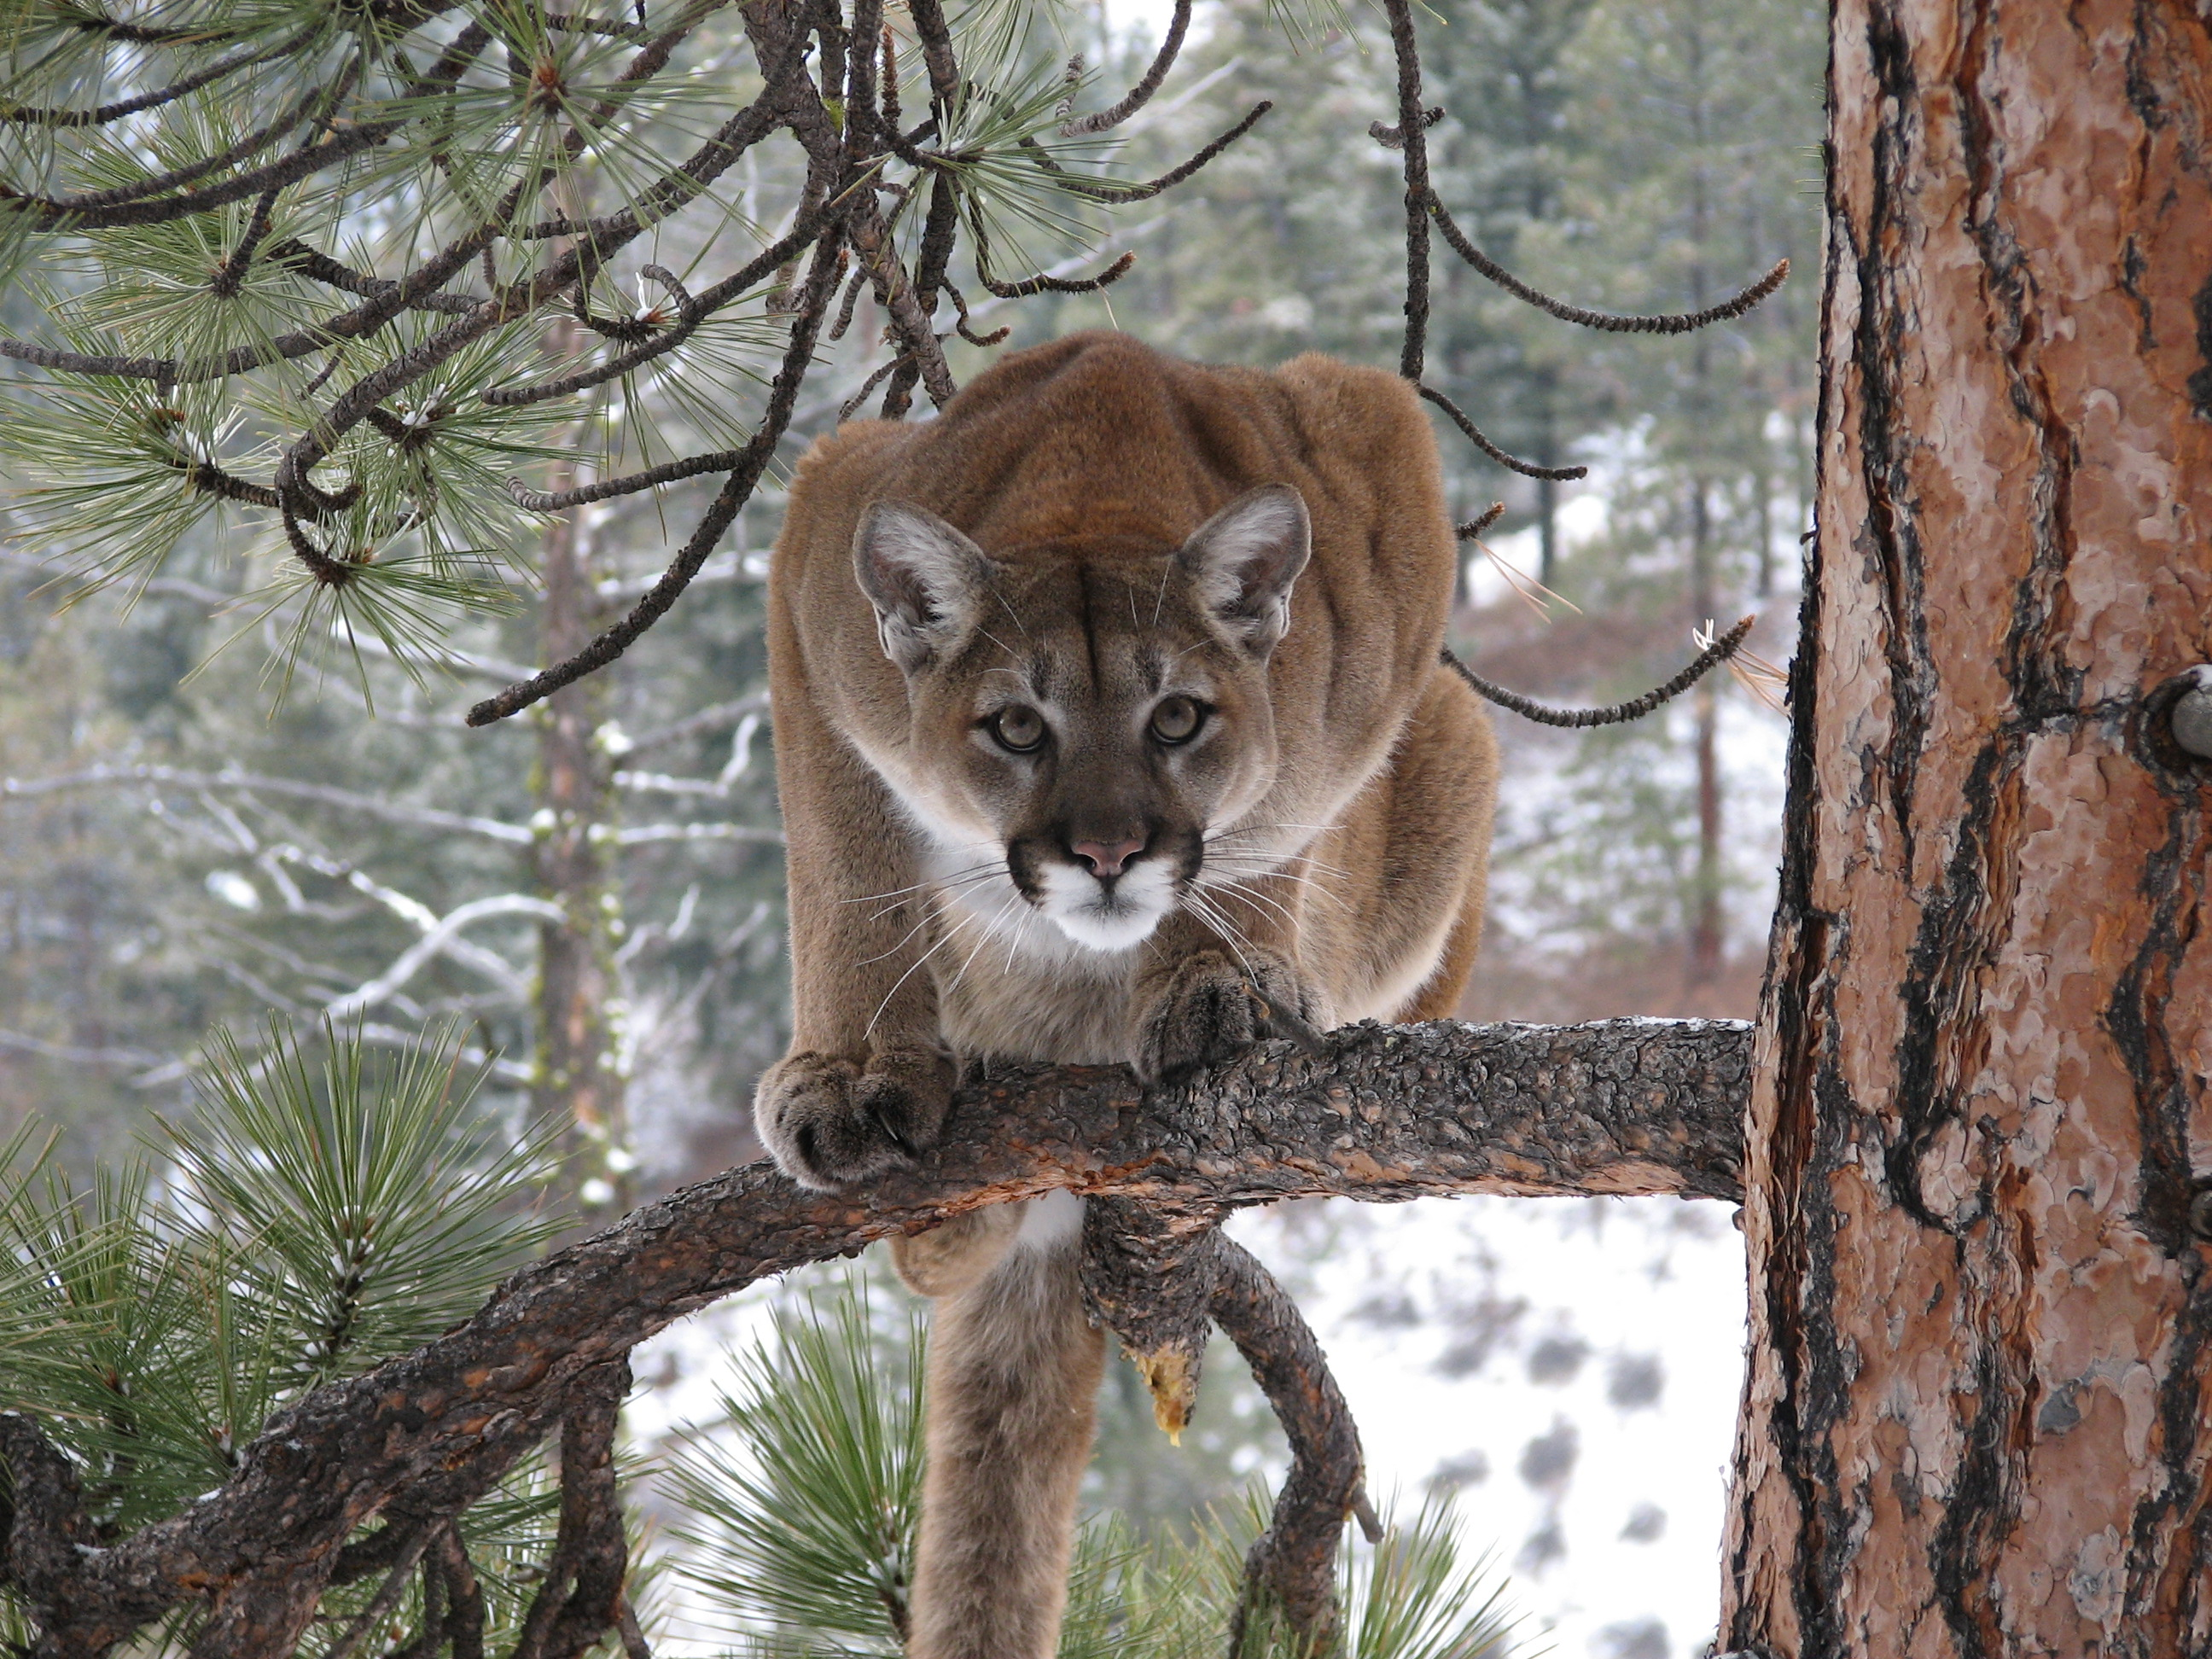
\includegraphics[height=3in]{Ch15-searchencounter/figs/mountain_lion.jpg}
\caption{
Mountain lion.
Run!
{\it Photo credit: Bob Wiesner}.
}
\label{searchencounter.fig.lion}
\end{figure}


\subsection{Sierra National Forest Fisher Study}

Here we consider a more detailed example and provide the data and
\R~script for this analysis.  The data come from an analysis of
individual encounter histories of the fisher ({\it Martes pennanti} by
\citet{thompson_etal:2012}.  The survey area was divided into 15
approximately 1,400 ha hexagons
(Fig. \ref{searchencounter.fig.fisherstudy}), which is roughly the
size of a female fisher's home range, and each hexagon was surveyed 3
times by sniffer dog teams searching space for scat. The dogs were
given considerably latitude to determine their route.  Thus, the
seearch path is not laid out a priori but rather evolves
opportunistically, based on what the dog senses at a local scale.  The
authors divided the region into 1 km grid cells (also shown in Fig.
\ref{searchencounter.fig.fisherstudy}).
We provide the 
data from this study
data(fisherdata) and the 
\R~function: \mbox{\tt SCRfisher} ..................

produces the following results:

Conclusions, thoughts, recommendations about this study...
What does this study show.............


%%% Andy: need to rerun
{\small
\begin{verbatim}
Inference for Bugs model at "modelfile.txt", fit using WinBUGS,
 3 chains, each with 6000 iterations (first 1000 discarded)
 n.sims = 15000 iterations saved
          mean    sd 2.5%   25%   50%   75% 97.5% Rhat n.eff
psi        0.5   0.3  0.1   0.3   0.5   0.8   1.0    1   110
sigma      4.8   2.9  0.2   2.3   4.8   7.3   9.7    1   820
N        269.7 140.0 26.0 153.0 265.0 394.0 497.0    1   110
lam0       0.0   0.0  0.0   0.0   0.0   0.0   0.0    1   200
alpha      0.2   0.2  0.0   0.1   0.1   0.3   0.6    1  3500
deviance  72.6   7.6 54.2  68.8  73.9  77.9  84.0    1   210

For each parameter, n.eff is a crude measure of effective sample size,
and Rhat is the potential scale reduction factor (at convergence, Rhat=1).

DIC info (using the rule, pD = var(deviance)/2)
pD = 28.8 and DIC = 101.4
DIC is an estimate of expected predictive error (lower deviance is better).
\end{verbatim}
}



\begin{figure}
\centering
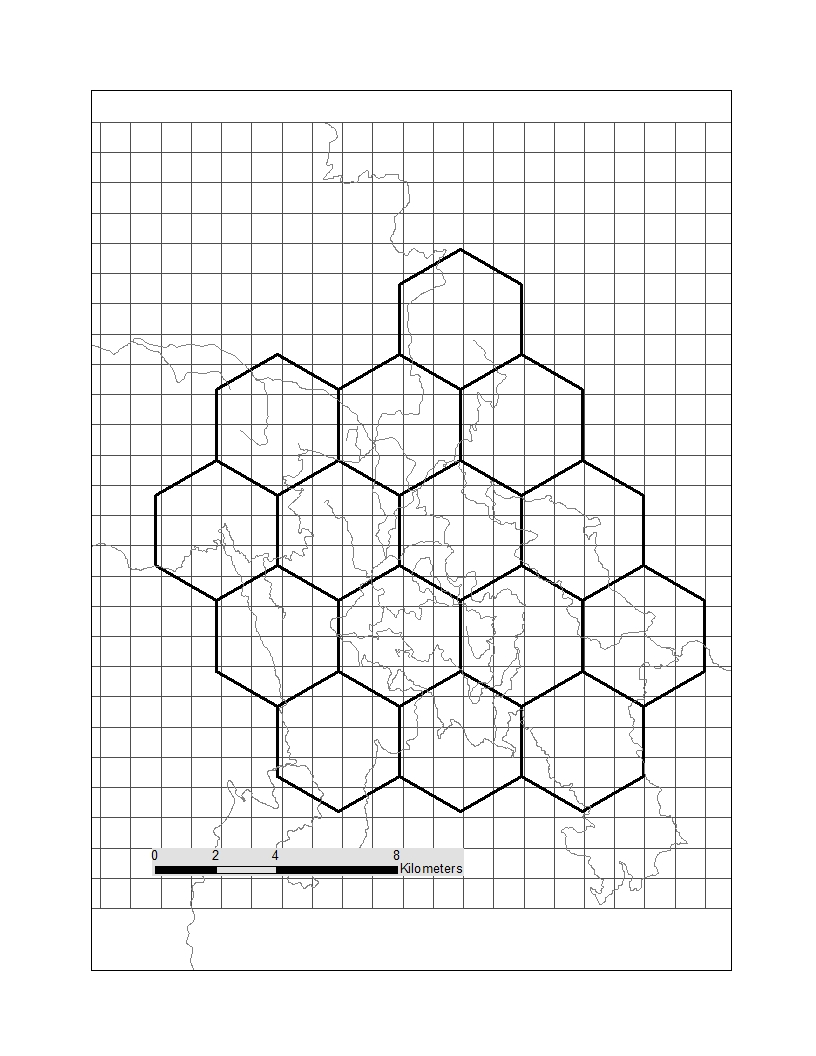
\includegraphics[width=2.3in]{Ch15-searchencounter/figs/fisher_map.jpg} 
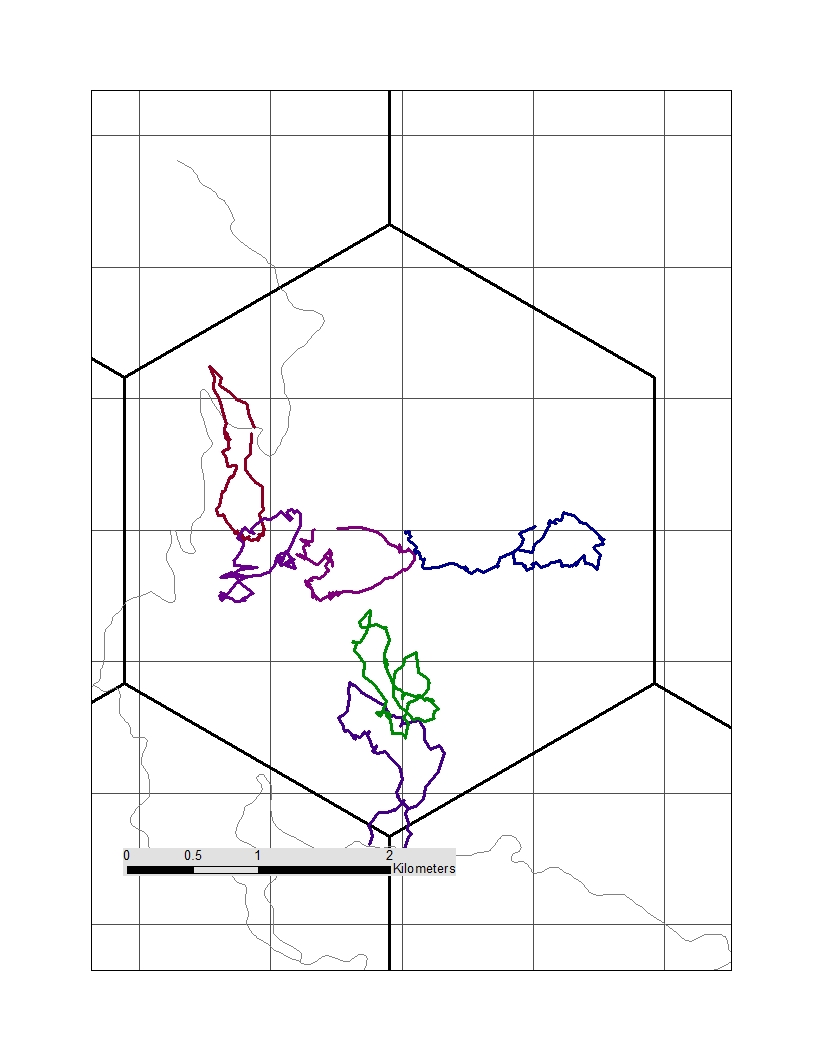
\includegraphics[width=2.3in]{Ch15-searchencounter/figs/fisher_tracklog.jpg} 
\caption{
Fisher study area showing the gridding system (left panel). The larger
hexagons are approximately the size of a typical female home
range. The 1 km grid cells define the SCR model grid, where the center
point of each one served as a trap. The right panel shows the GPS
trackline of the dog team through one of the grid cells. The total
length of the trackline was used as a covariate on encounter probability.
{\it Credit: Craig Thompson, U.S. Forest Service}
}
\label{searchencounter.fig.fisherstudy}
\end{figure}






\section{Design 2: Uniform Search Intensity}

A special case of a search-encounter type of model arises when it is
possible to subject a quadrat (or quadrats) to a uniform search
intensity. This could be interpreted as an exhaustive search, or
perhaps just a thorough systematic search of the avaialable habitat.
The example considered by \citet{royle_young:2008} involved searching
 a 9 ha plot for horned lizards (Fig.
\ref{searchencounter.fig.hornylizard}) by a crew of several people. It
was felt in that case that complete and systematic (i.e., uniform) coverage of the plot was
achieved. In general, however, we think you could have a random sample
of the plot and approximate that as a uniform coverage -- this is kind
of a design-based argument justifying the uniform search intensity
model (we haven't simulated this situation, but it would be worth
investigating).

\begin{figure}[ht]
\centering
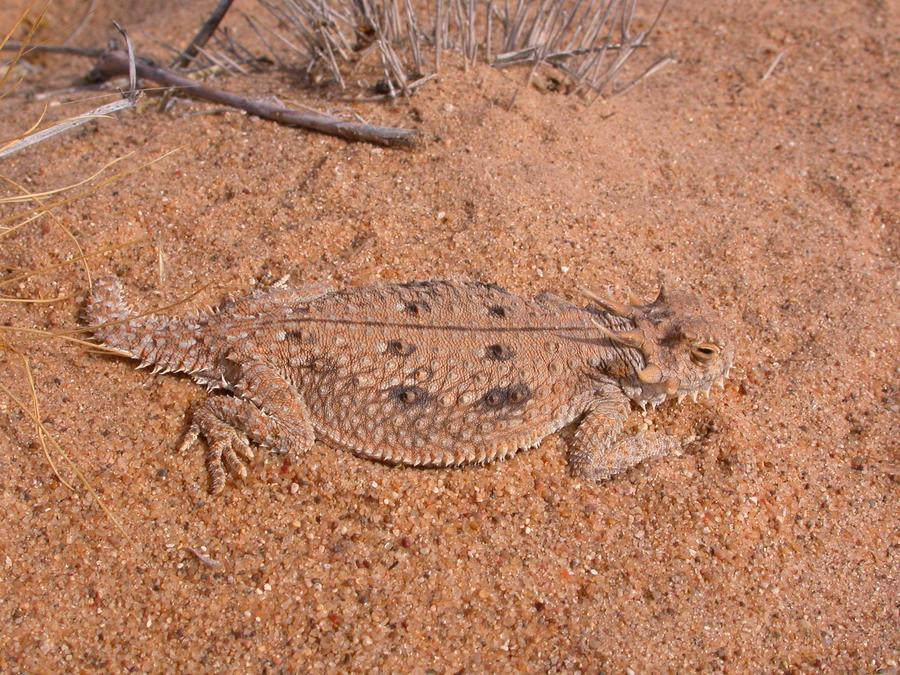
\includegraphics[width=3.6in,height=2.7in]{Ch15-searchencounter/figs/horny_lizard.jpg}
\caption{A flat-tailed horned lizard showing its typical cryptic
  appearance in its native environment.  Detection of flat-tailed
  horned lizards is difficult because they do not run when
  approached. Instead they shuffle under the sand or press down and
  remain motionless as shown in the picture.  The horns are employed
  only as a last resort if the camouflage fails.  {\it Photo credit:
    Kevin and April Young} }
\label{searchencounter.fig.hornylizard}
\end{figure}

It is clear that this uniform search intensity model is a special case
of the more general search-encounter model in the sense that the
probability of encounter of an individual is a constant $p_{0}$ {\it
  if} the individual is located in the polygon ${\cal X}$ during
sample occasion $k$, i.e.,
\[
p({\bf u}_{ik}) = p_{0} \mbox{I}({\bf u}_{ik} \in {\cal X})
\]
which resembles Eq. \ref{search-encounter.eq.hardplot} except
replacing the encounter probability function with constant $p_{0}$.

Subsequently, we give a simple analysis using simulated data and 
simple movement models for ${\bf u}$, including a bivariate normal
model and a random walk. 
For further examples and analyses, we refer you to
\citet{royle_dorazio:2008}, who reanalyzed the lizard data from
\citet{royle_young:2008}, and \citet{efford:2011ecol} and
\citet{marques_etal:2011}.



\subsection{Alternative movement models}
\label{searchencounter.sec.movement}

As with the general search-encounter model (``Design 1''), we require
a model to describe the movement outcomes ${\bf u}_{ik}$.
In the analysis of \citet{royle_young:2008}, a simple bivariate
Gaussian movement model was used, in which
\[
 {\bf u}_{ik} | {\bf s}_{i} \sim \mbox{Normal}({\bf s}_{i}, \sigma^{2}{\bf I}),
\]
However, clearly more general versions of the model can be developed.
For example, imagine a situation where the successive surveys of a
bounded sample polygon are relatively close together in time so that
successive locations of individuals are not well-approximated by the
Gaussian movement model, which implies independence of
locations. Naturally we might consider using an auto-regressive or
random-walk type of model in which the successive coordinate locations
of individual $i$ behave as follows:
\begin{eqnarray*}
 u_{1,i,k} | u_{1,i,k-1} &\sim &  \mbox{Normal}( u_{1,i,k-1},  \sigma^{2}) \\
 u_{2,i,k} | u_{2,i,k-1} &\sim &  \mbox{Normal}( u_{2,i,k-1},  \sigma^{2}) \\
\end{eqnarray*}
here we use the notation $u_{1}$ and $u_{2}$ for the easting and
northing coordinates, respectively. (and, for clarity, we are using
commas in the sub-scripting here when we have to refer to time-lags).
 In addition, we require that the initial locations have a
distribution and, for that, we might begin with a simple model such as
the uniformity model:
\[
 {\bf u}_{i,1} \sim \mbox{Uniform}({\cal S})
\]
which effectively takes the place of the model for ${\bf s}_{i}$ that
we typically use. Under this model, individuals don't have an activity
center but, rather, they drift through space more-or-less randomly
based just on their previous location. See \citet{ovaskainen:2004} and
\citet{ovaskainen_etal:2008} for development and applications of similar
movement models in the context of capture-recapture data,
and also our discussion of a similar model that might arise in
acoustic surveys (Sec. \ref{poisson-mn.sec.acoustic}).  We could allow
for dependent movements about a central location ${\bf s}_{i}$ using a
bivariate auto-regression or similar type of model with parameter
$\rho$, e.g.,
\[
 {\bf u}_{i,k} | {\bf s}_{i} \sim   \mbox{BVN}( \rho*( {\bf u}_{i,k-1} - {\bf s}_{i} ),  \sigma^{2} {\bf I}).
\]

We don't have any direct experience fitting these movement models to
real capture-recapture data, but we imagine they should prove
effective in applications that yield large sample sizes of individuals
and recaptures. 

\subsection{Simulating and fitting uniform search intensity models}

The {\bf R} script \mbox{\tt uniform\_search}, in the \mbox{\tt scrbook} package, we provide a script for simulating
and fitting search-encounter data using the iid Gaussian model and
also the random walk model.  The {\bf BUGS} model specification is
shown in Panel \ref{search-encounter.panel.uniform} for the random
walk situation. We encourage you to adapt this model and the
simulation code for the auto-regression movement model.  To fit this
model to data, we set up the run with {\bf JAGS} using the standard
commands. We did not specify starting values for the missing
coordinate locations although we imagine that {\bf JAGS} should
perform better if we provide decent starting values, e.g., the last
observed location or some other reasonable location.  We imagine that
resource selection could be parameterized in this movement model as
well, perhaps using similar ideas to those described in
Chapt. \ref{chapt.rsf}.

The following script simulates a population of N individuals and their
locations at each of 4 times to see if they are in a square [3,13] or
not.  This simulates a random walk thing so we imagine that the
sampling occasions are close together in time.  The initial state is
assumed to be uniformly distributed on the state-space which, in this
case, is the square $[0,16] \times [0,16]$.

{\small
\begin{verbatim}
> N <- 100
> nocc <- 4
> Sx <- Sy <- matrix(NA,nrow=N,ncol=nocc)
> sigma.move <- .25

# simulate initial coordinates on the square:
> Sx[,1] <- runif(N,0,16)
> Sy[,1] <- runif(N,0,16)

> for(t in 2:nyear){
+    Sx[,t] <- rnorm(N,Sx[,t-1],sigma.move)
+    Sy[,t] <- rnorm(N,Sy[,t-1],sigma.move)
+ }

# now we generate encounter histories:
> f <- rep(NA,N)
> Y <- matrix(0,nrow=N,ncol=nyear)
> for(i in 1:N){
+   for(t in 1:nyear){
+     # IF individual is IN THE SQUARE we can capture it:
+     if( Sx[i,t] > 3 & Sx[i,t]< 13 & Sy[i,t]>3 & Sy[i,t]<13 )
+     Y[i,t] <- rbinom(1,1,.5)
+   }
+   # f[i] = 1 period of 1st capture, NA if never captured
+   if(sum(Y[i,])>0)
+    f[i] <-  min((1:nyear)[Y[i,]==1][1])
+ }

# Subset data. If a guy is never captured, cannot have him in our data set

> Y <- Y[!is.na(f),]
> Sx <- Sx[!is.na(f),]
> Sy <- Sy[!is.na(f),]

> Sx[Y==0] <- NA
> Sy[Y==0] <- NA

## Data augmentation:
> M <- 200
> Y <- rbind(Y,matrix(0,nrow=(M-nrow(Y)),ncol=nyear))
> Sx <- rbind(Sx,matrix(NA,nrow=(M-nrow(Sx)),ncol=nyear))
> Sy <- rbind(Sy,matrix(NA,nrow=(M-nrow(Sy)),ncol=nyear))

# Make 3-d array of coordinates
> G <- array(NA,dim=c(M,nyear,2))
> G[,,1] <- Sx
> G[,,2] <- Sy
\end{verbatim}
}

\begin{panel}[htp]
\centering
\rule[0.15in]{\textwidth}{.03in}
{\small
\begin{verbatim}
model{
psi ~ dunif(0,1)
tau ~ dgamma(.1,.1)
p0 ~ dunif(0,1)
sigma.move <- sqrt(1/tau)

# Likelihood
for (i in 1:M){
  z[i] ~ dbern(psi)
  G[i,1,1] ~ dunif(0,16)
  G[i,1,2] ~ dunif(0,16)

   for (t in 2:n.occasions){
## See here I can only make a model for LOCATION
      G[i,t,1] ~ dnorm(G[i,t-1,1], tau)
      G[i,t,2] ~ dnorm(G[i,t-1,2], tau)
    }
   for(t in 1:n.occasions){
            # Test whether the actual location is in- or outside the
            #     survey area. Needs to be done for each grid cell

      inside[i,t] <- step(G[i,t,1]-3) * step(13-G[i,t,1]) *
                     step(G[i,t,2]-3) * step(13-G[i,t,2])
      Y[i,t] ~ dbern(mu2[i,t])
      mu2[i,t] <- p0 * inside[i,t] * z[i]
      } #t
   } #i
N <- sum(z[])
}
\end{verbatim}
}
\rule[-0.15in]{\textwidth}{.03in}
\caption{
{\bf BUGS} model specification for the search-encounter model similar
to Royle and Young (2008) but with a random walk movement model.
help file \mbox{\tt ?uniform$\_$search} in the {\bf R} package \mbox{\tt scrbook}.
}
\label{search-encounter.panel.uniform}
\end{panel}

\subsection{Movement and Dispersal in Open Populations}

In Chapt. \ref{chapt.open} we discuss many aspects of modeling open
populations, including some aspects of modeling movement and dispersal
and the relevance of SCR models to these problems. However, given the
introduction of the search-encounter model above, this is celarly
relevant to modeling movement and dispersal in open populations.  In
particular, the model described in Panel
\ref{search-encounter.panel.uniform} could easily be adapted to an
open population by conditioning on the first, and introducing a latent
``alive state'' with survival parameter $\phi_{t}$. This would be a
spatial version of the standard Cormack-Jolly-Seber model
(Chapt. \ref{open.sec.cjs})\footnote{Some work related to this is
  currently being carried out by our colleagues Torbj{\o}rn Ergon and
  Michael Schaub.}.


\section{Partial Information Designs}

The prototype search-encounter (Design 1) and uniform search (Design
2) cases are ideal in the sense that they product both precise
locations of individuals and also a precise characterization of the
manner in which individuals are encountered by sampling space.  We
have seen a number of studies that, in an ideal world, would have
generated data consistent with one of these situations but, for some
practical reason or other reason, partial or no spatial information
about the search area or the locations of individuals was collected
(or retained), and so the models described above could not be used.
We imagine at least 
3 distinct situations

\begin{itemize}
\item[(a)] The search path is not recorded, but locations  of
  individuals are recorded 
\item[(b)] The search path is recorded, but locations of individuals
  are not.
\item[(c)] The search path is not recorded, and the locations are not
  recorded, just the raw counts.
\end{itemize}

For analysis of these search-encounter designs with partial information,
we see a number of options of varying levels of formality,
depending on the situation (and these are largely untested). 
For (a) You could always assume uniform search intensity,
which might be reasonable if the plots were randomly
searched. Otherwise, its validity would depend on the precise manner
in which the search activity occurred. 
For (b) or (c), we could adopt the approach we took in the fisher analysis
above, and  map the locations to the center of each plot, thinking of
the plot as an effective trap, and using the search path length
as a covariate.

A 4th case of even less information is that in which 
we don't record individual identity at all. Instead, 
we just have total count frequencies in each plot.
This model is precisely the one considered by
\citep{chandler_royle:2012} and this is the focus of
Chapt. \ref{chapt.scr-unmarked}.
% XXXX RC: In Ch18, I now have something of a search-encounter model for
% Evan's salamander data where stream segments are uniformly search
% and sampled using removal sampling.















\begin{comment}
\subsection{Capricaillie status in Switzerland}

Variations of models with partial information have appeared in a
number of papers.  One of those is \citet{mollet_etal:2012}, who obtained a population
size estimate of a large forest grouse species
(Fig. \ref{searchencounter.fig.capercaillie}) known as the
capracaillie ({\it Tetrao urogallus}) in Switzerland.  
Forest
stands were searched by observers for scat, which was analyzed for DNA
identification of individuals.  A total of 78 spatial units of a few
ha each were searched.  In this example, forest stands were searched
but the search path data was not available, only the unit in which
each scat was found.  It was searched in an expert manner, and it was
believed that a uniform search intensity model could be reasonable.
\citet{mollet_etal:2012} used a basic Poisson
SCR model (Chapt. \ref{chapt.poisson-mn}). 

Importantly,
the sample units are actually large forest patches on the order of
tens of hectares each, but variable in size. Data were {\it not} collected
by coordinates of observations but rather just recorded to the
specific patch in which the observation was encountered. To accomodate
this we defined ${\bf s}_{i}$ to be a discrete random variable taking
on the centroid of each of the 1-78 forest fragments. 
Forest patches were searched for scat which was situation
in which discrete patches of habitat are searched using some method
and it might be convenient (or occur inadvertently) to associate
samples to the patch level instead of recording observation
locations. In this case we might use a model
$s[i] \sim dcat(probs[])$ % XXXX Seems to be hybrid BUGS/stats notation
where $probs[]$ are the probabilities that an individual inhabits a
particular patch.



\begin{figure}
\centering
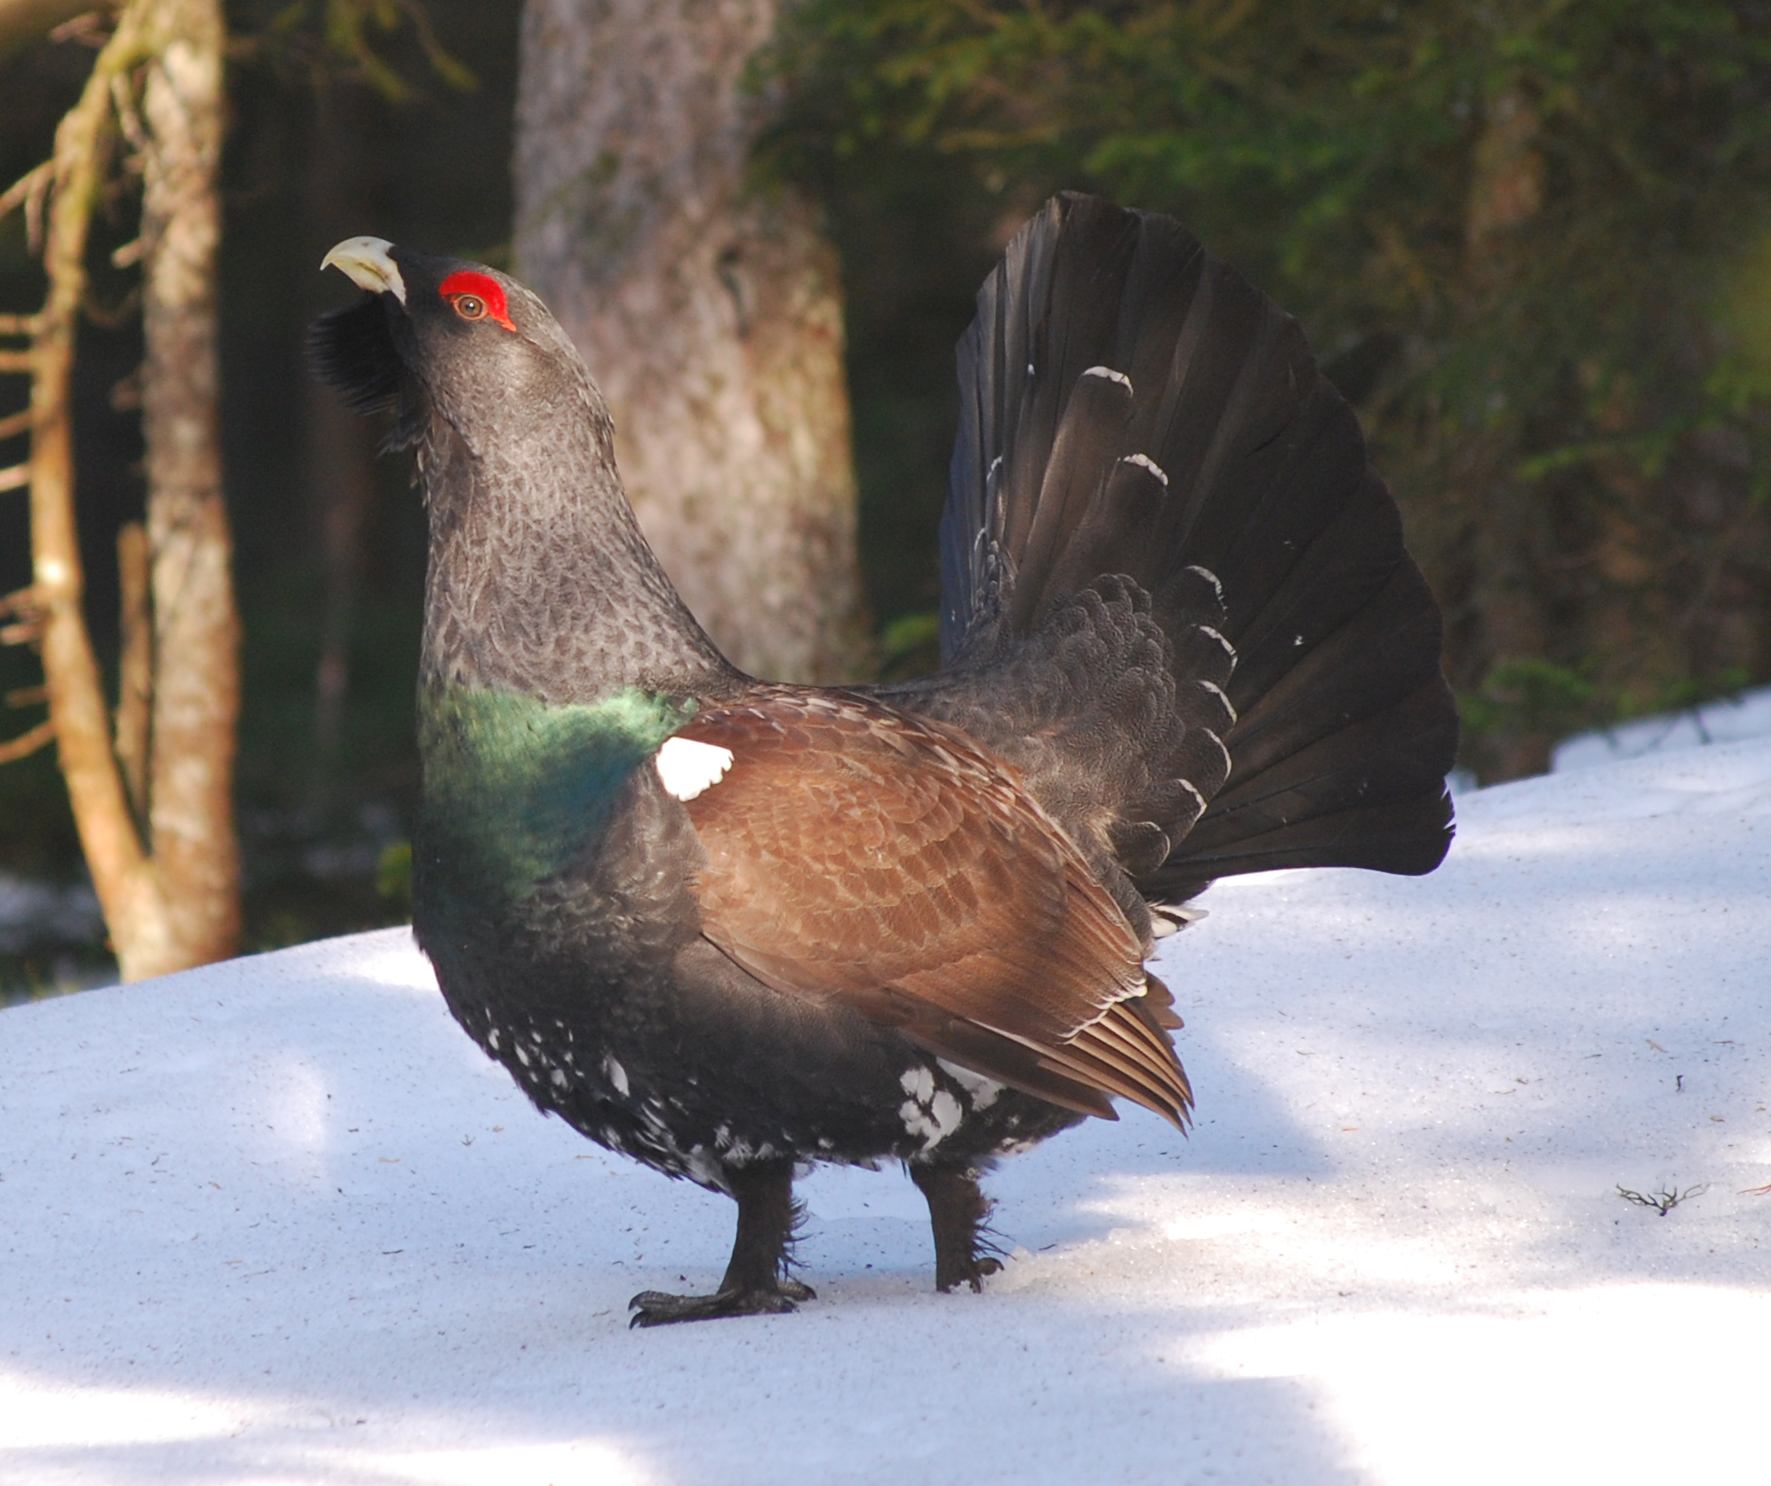
\includegraphics[width=5in,height=4.21in]{Ch15-searchencounter/figs/capercaillie_lanz.jpg}
\label{searchencounter.fig.capercaillie}
\caption{A male caprcaillie in its typical lekking position,
{\it Photo credit: Michael Lanz, Switzerland}.
}
\end{figure}

A discrete state-space model was used in which
activity centers were uniformly distributed to each
of the 78 fragments in proportion to area of the forest patch within
which each fragment was located.  This is similar to the multi-session
formulation of the model where, in this case, the ``sessions'' are
discrete forest fragments but, unlike the multi-session models above,
the encounters of an individual can occur in multiple sessions.  The
authors assumed that
\[
 N_{f} \sim \mbox{Poisson}( A_{f} \lambda_{0} )
\]
where $N_{f}$ is the population size for fragment $f$, 
which implies (see Chapt. \ref{chapt.hscr}):
\[
{\bf s}_{i} \sim  \mbox{Categorical}(  \pi_{f} )
\]
with
\[
 \pi_{f} = \frac{ \lambda_{f} }{\sum_{f} \lambda_{f}}
\]
The observation model: Each of the 78 fragments is its own sample unit
which we index to the center point of the fragment. No finer scale
information is made about the observation locations.  Let $y_{ij}$ be
the number of times individual $i$ encountered in stand $j$.
\end{comment}


\section{Summary and Outlook}

The generation of spatial encounter history data in ecological studies
is widespread. While such data have historically been obtained mostly
by the use of arrays of fixed traps (catch traps, camera traps,
etc..), in this chapter we showed that SCR models are equally relevant
to a large class of ``search-encounter'' problems (we used the term
``designs'' in an attempt to provide a taxonomy of distinct cases of
search-encounter surveys) which are based on organized or
opportunistic searches of spatial areas. A standard example is that in
which detector dogs are used to obtain scat samples, from which DNA
can be obtained to determine individual identity.  Another example is
that in which a fixed survey path, or collection of transects, is
surveyed by an observer and the locations of detected individuals are
recorded (this is common in sampling for reptiles and amphibians). 
The latter situation closely resembles distance sampling,
but with repeated observations of the same individual (on multiple
occassions) it has a distinct capture-recapture element to it. In a
sense, some of these search-encounter models are hybrid SCR-DS models.

Many models for search-encounter data have three elements in common:
(1) They contain a model for encounter conditional on locations of
individuals; (2) a model that describes how these observable animal
locations are distributed in space about their activity centers; and
(3) a model for the distribution of activity centers.  We interpret
the 2nd model component as an explicit movement model, and the
existance of this component is distinct from most of the other models
considered in this book.
%Thus, search encounter models
%are somewhat more general than the standard SCR models
%where observations are restricted to a priori fixed locations.

One of the key conceptual points is that, with these search-encounter
types of designs, the locations of observations are {\it not} biased
by the locations of traps but, rather, locations of individuals can
occur anywhere within search plots or quadrats, or in the vicinity of
a transect or search path.  Because we can obtain direct observations
of location -- outcomes of movement -- for individuals, it is possible
to resolve explicit models of movement from search-encounter data.  We
considered the simple case of the independent bivariate normal
movement model, and also a random walk type model, which can easily be
fitted in the {\bf BUGS} engines.  We imagine much more general
movement models can be fitted, although we have had limited
opportunities to pursue this and in most practical capture-recapture
studies, we will probably be limited by sparse data in the complexity
of the movement models that could be considered.

Search encounter type of sampling seems to be fairly common, although
we think that many people don't realize that it can produce encounter
history data that is amenable to the development of formal models for
density, movement and space usage. We believe that these protocols
will become more appealing as methods for formal analysis of the
resulting encounter history data become more widely known.  At the
same time, search-encounter models will prove to be enormously useful
in future studies of animal populations because so many new methods of
obtaining encounter history data can be be based on DNA extracted from
animal tissue or scat, which is easy to obtain by searching space and
collecting it opportunistically.  In addition, as the cost of
extracting individual identity from scat or tissue decreases, its
widespread collection and use in capture-recapture models can only
increase.
